%!TEX TS-program = xelatex
\documentclass{beamer}

\usepackage{HSE-theme/beamerthemeHSE-en} % Load HSE theme

%%% Fonts 
\usepackage{fontspec}
\defaultfontfeatures{Ligatures={TeX},Renderer=Basic}
\setmainfont[Ligatures={TeX,Historic}]{Myriad Pro} % install Myriad Pro or replace with Arial
\setsansfont{Myriad Pro}  % install Myriad Pro or replace with Arial
\setmonofont{Courier New}

\usepackage{multicol} 		% Multiple columns
\graphicspath{{images/}}  	% Images folder

%%% Author and speech
\title[Short title]{Network Science Project 1} 
\subtitle{ Network Analysis of Emails Sent Within Enron}
\author[Frank Acquaye]{Presented By \\ \smallskip \scriptsize \url{fakvey@edu.hse.ru}\\\url{http://acquayefrank.github.io/}}
\institute[Higher School of Economics]{National Research University \\ Higher School of Economics (Moscow)}
\date{\today}

\begin{document}	% Document begins

\frame[plain]{\titlepage}	% Title frame

%\section{Just some text}
%\subsection{Subtitle}

\begin{frame}
\frametitle{Network Summary Part 1}
	\begin{multicols}{2}
		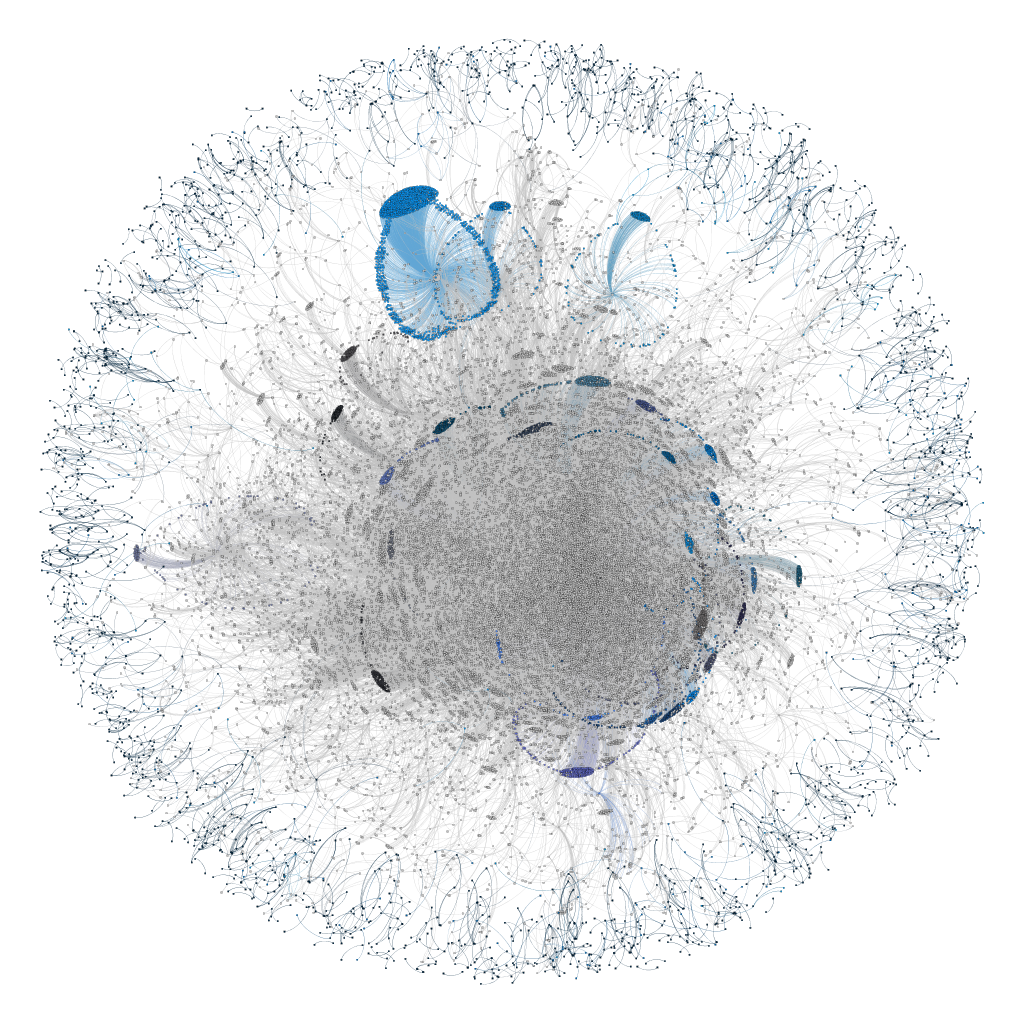
\includegraphics[width=\columnwidth]{na-ee-graph-final.png}
		\columnbreak

		\begin{enumerate} 
			\item \textbf{Nodes/Order:} 36692
			\item \textbf{Edges/Size:} 183831
			\item \textbf{Radius:} 7
			\item \textbf{Diameter:} 13		
			\item \textbf{Transitivity:}  0.085
			\item \textbf{Clustering Co-efficient:} 0.497
		\end{enumerate} 
	\end{multicols}
\end{frame}

\begin{frame}
\frametitle{Network Summary Part 2}
	\begin{multicols}{2}
		\begin{figure}
	        {\tiny Scatter Plot of Degree Distribution}
		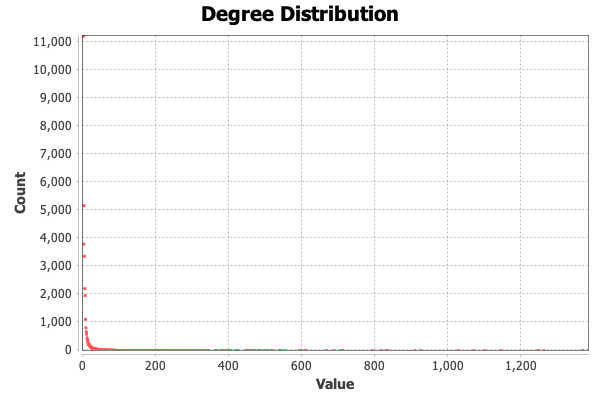
\includegraphics[width=\columnwidth]{degree-distribution.png}
		\end{figure}
		\columnbreak
		\begin{figure}
		{\tiny Scatter Plot of  Weighted Degree Distribution}
		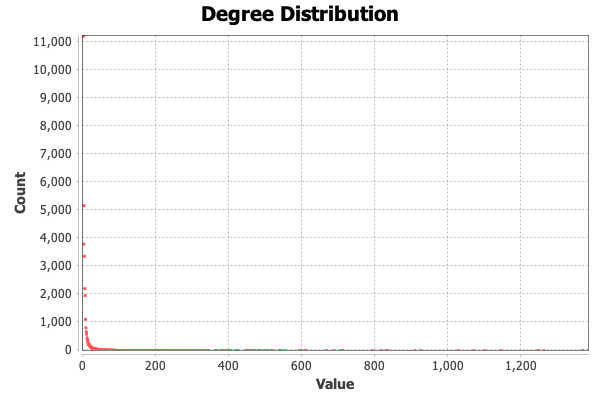
\includegraphics[width=\columnwidth]{w-degree-distribution.png}
		\end{figure}
	\end{multicols}
\end{frame}

\begin{frame}
\frametitle{Structural Analysis Part 1}
	\begin{multicols}{2}
		\begin{figure}
	        {\tiny Bar Chart of Degree Centrality Measure}
		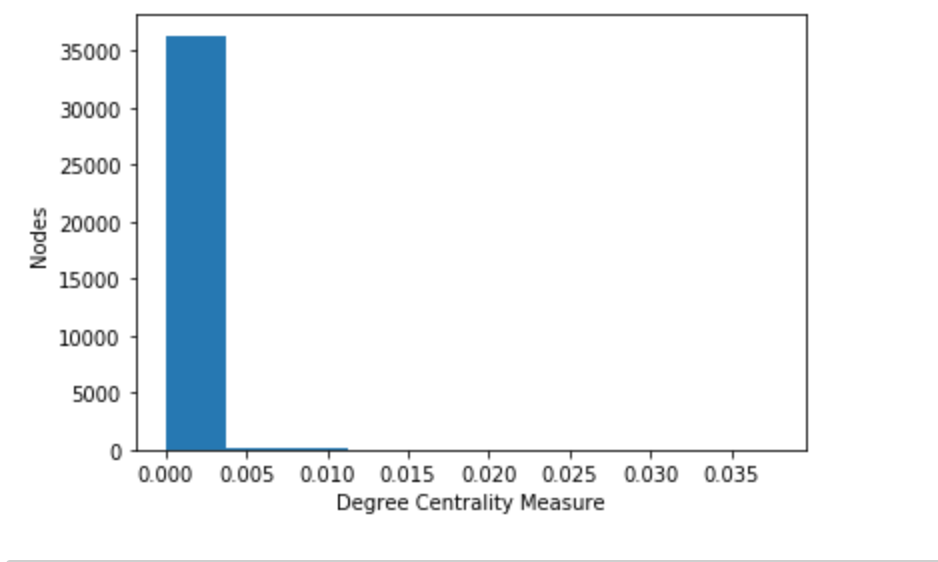
\includegraphics[width=\columnwidth]{degree-cent.png}
		\end{figure}
		\columnbreak
		{\tiny Top Five Nodes according to Degree Centrality} \\
		Node  ->  Measure
		\begin{enumerate} 
		\item \textbf{5038} -> 0.0376
		\item \textbf{273} -> 0.0372
		\item \textbf{458} -> 0.0343
		\item \textbf{140} -> 0.0339
		\item \textbf{1028} -> 0.0339
		\end{enumerate} 
	\end{multicols}
\end{frame}

\begin{frame}
\frametitle{Structural Analysis Part 2}
	\begin{multicols}{2}
		\begin{figure}
	        {\tiny Bar Chart of Closeness Centrality Measure}
		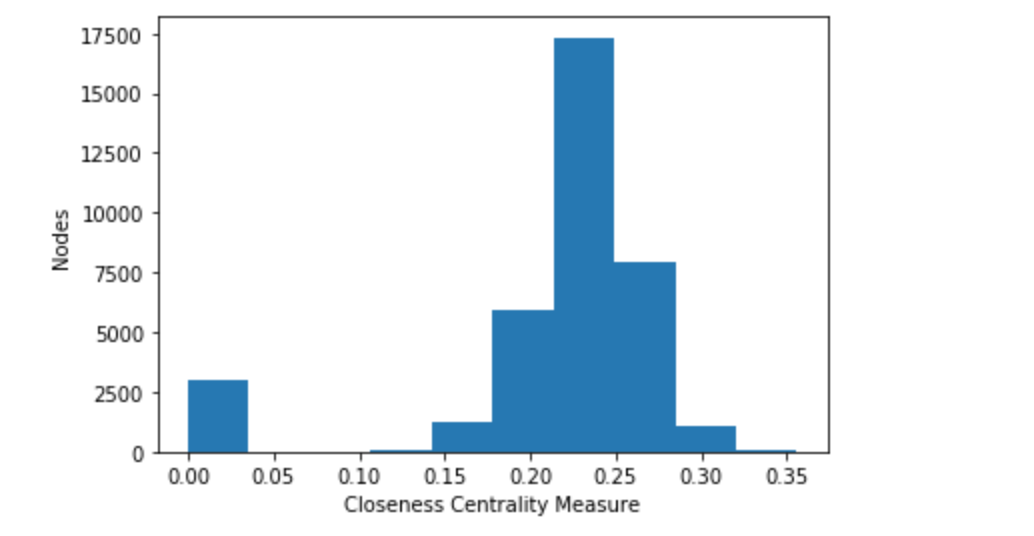
\includegraphics[width=\columnwidth]{close-cent.png}
		\end{figure}
		\columnbreak
		{\tiny Top Five Nodes according to Degree Centrality} \\
		Node  ->  Measure
		\begin{enumerate} 
		\item \textbf{136} -> 0.3557
		\item \textbf{76} -> 0.3546
		\item \textbf{46} -> 0.3481
		\item \textbf{140} -> 0.3441
		\item \textbf{370} -> 0.3439
		\end{enumerate} 
	\end{multicols}
\end{frame}


\begin{frame}
\frametitle{Structural Analysis Part 3}
	\begin{multicols}{2}
		\begin{figure}
	        {\tiny Bar Chart of Betweeness Centrality Measure}
		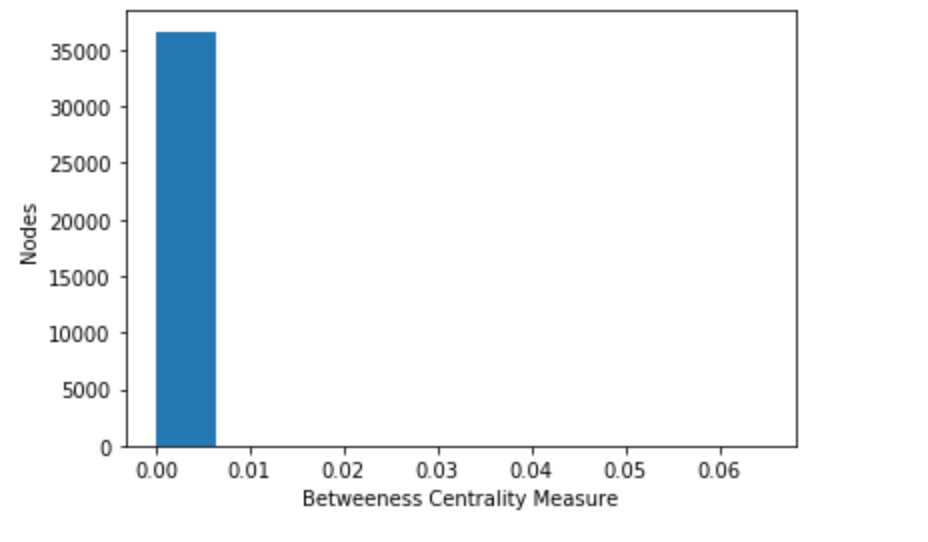
\includegraphics[width=\columnwidth]{between-cent.png}
		\end{figure}
		\columnbreak
		{\tiny Top Five Nodes according to Degree Centrality} \\
		Node  ->  Measure
		\begin{enumerate} 
		\item \textbf{5038} -> 0.0648
		\item \textbf{140} -> 0.0604
		\item \textbf{566} -> 0.0363
		\item \textbf{588} -> 0.0354
		\item \textbf{1139} -> 0.0354
		\end{enumerate} 
	\end{multicols}
\end{frame}


\begin{frame}
\frametitle{Structural Analysis Part 4}
	\begin{multicols}{2}
		\begin{figure}
	        {\tiny Bar Chart of Page-Rank}
		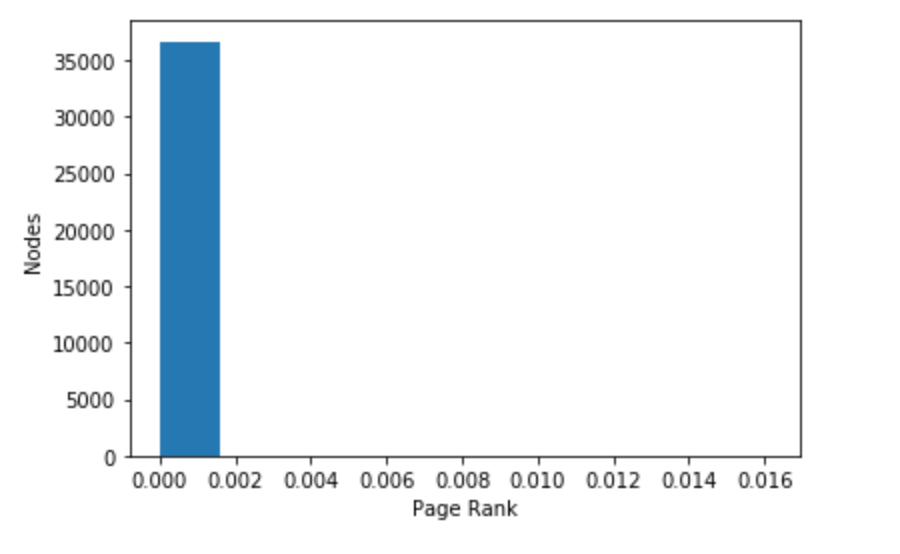
\includegraphics[width=\columnwidth]{page-rank.png}
		\end{figure}
		\columnbreak
		{\tiny Top Five Nodes according to Degree Centrality} \\
		Node  ->  Measure
		\begin{enumerate} 
		\item \textbf{5038} -> 0.0161
		\item \textbf{273} -> 0.0033
		\item \textbf{588} -> 0.0032
		\item \textbf{566} -> 0.0030
		\item \textbf{140} -> 0.0029
		\end{enumerate} 
	\end{multicols}
\end{frame}

\begin{frame}
\frametitle{Structural Analysis Part 5}
	\begin{center}
	 	{\tiny Assortative Mixing and Structural Similarity of top 250 Nodes according to page rank}
	\end{center}
	 \begin{figure}
		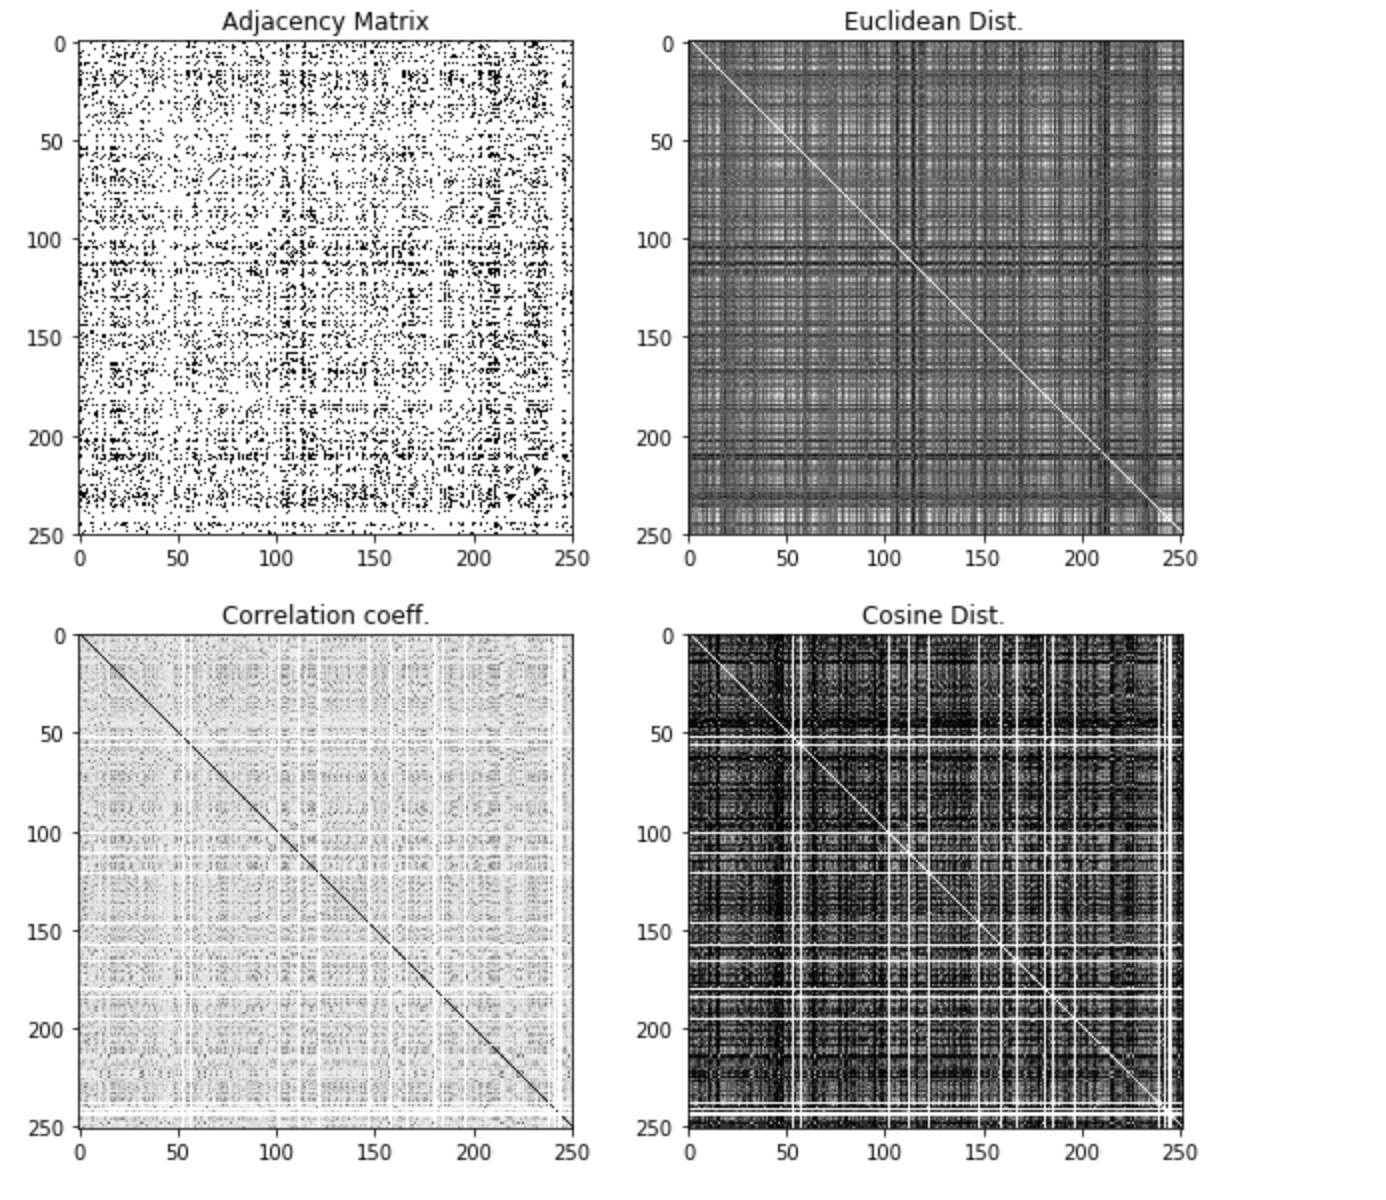
\includegraphics[width=75mm]{adj.png}
	\end{figure}
\end{frame}

\begin{frame}
\frametitle{Community Detection Part 1}
	\begin{center}
	 	{\tiny Largest Clique}
	\end{center}
	 \begin{figure}
		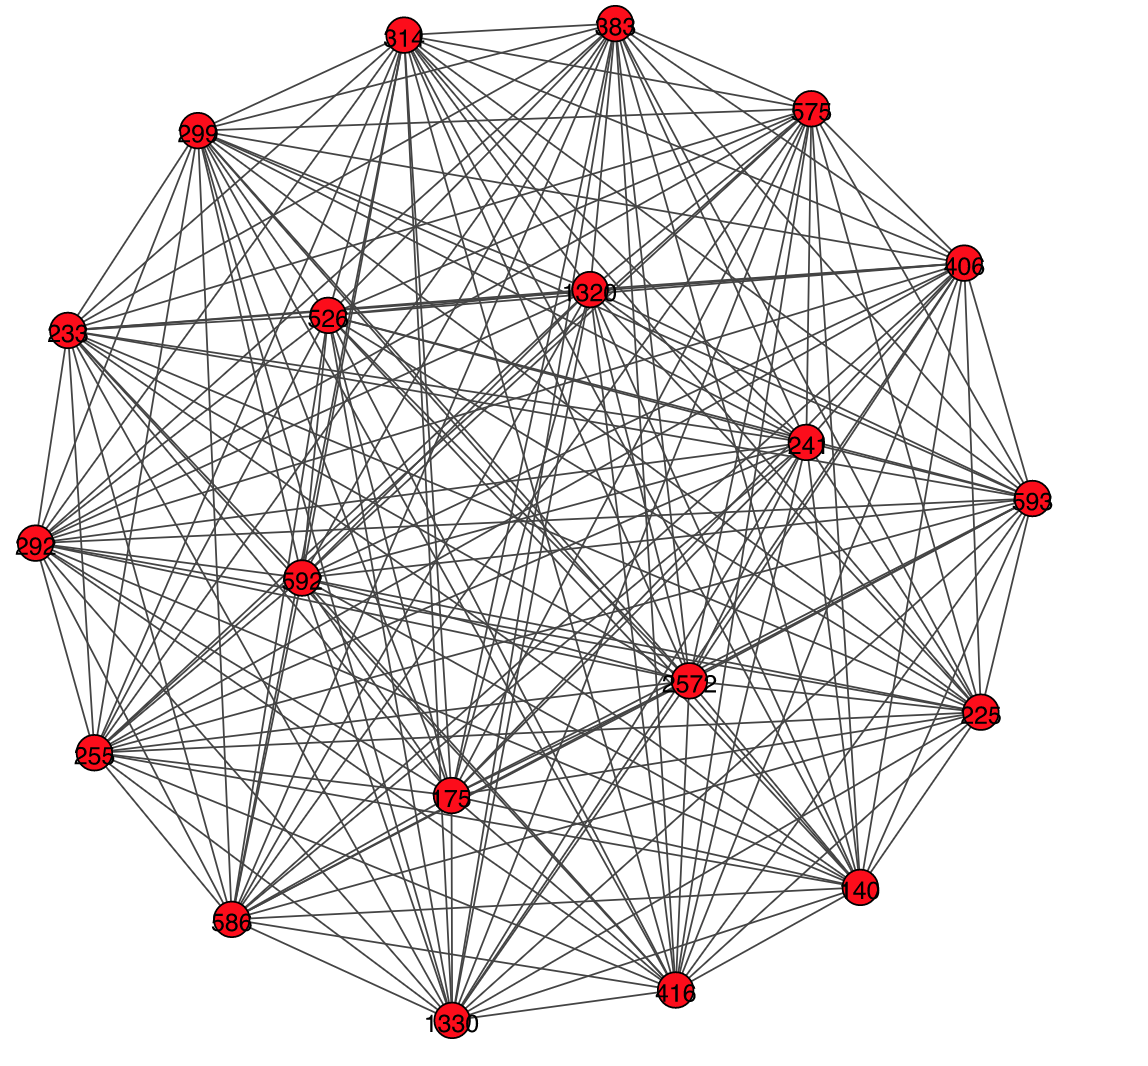
\includegraphics[width=70mm]{clique-search.png}
	\end{figure}
\end{frame}

\begin{frame}
\frametitle{Community Detection Part 2}
	\begin{center}
	 	{\tiny Community Detection of top 250 Nodes according to page rank}
	\end{center}
	 \begin{figure}
		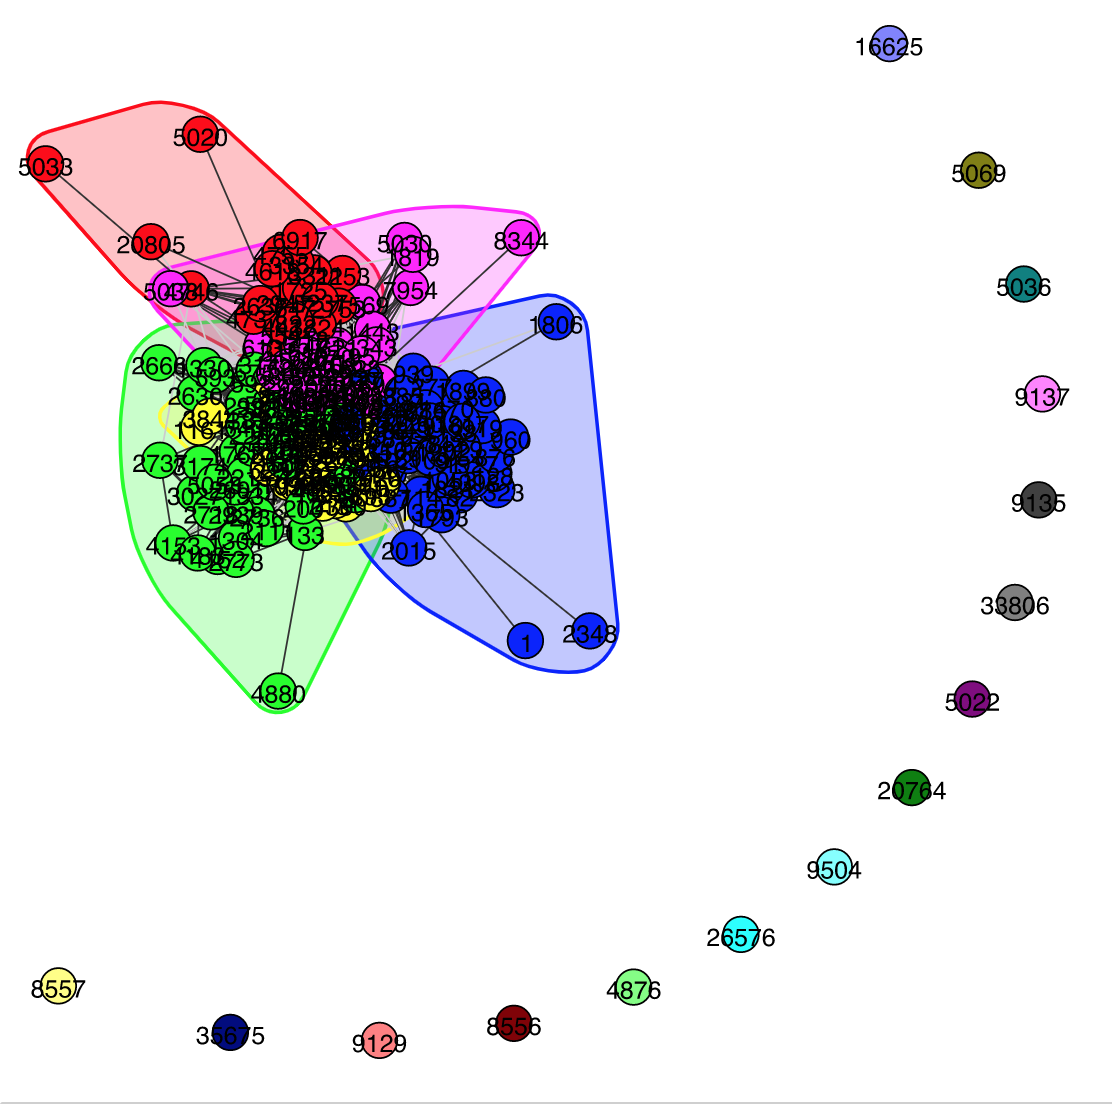
\includegraphics[width=70mm]{communities-page-rank.png}
	\end{figure}
\end{frame}


\begin{frame}[c]
\begin{center}
\frametitle{\LARGE Thank you for your attention!}

{\LARGE \inserttitle}

\bigskip

{\insertauthor} 

\bigskip\bigskip

{\insertinstitute}

\bigskip\bigskip

{\large \insertdate}
\end{center}
\end{frame}

\end{document}